W dalszej części rozdziału skupimy się już tylko na komponentach spreadu, ponieważ to one, a nie sam spread będą modelowane. W ramach EDA dokonaliśmy standardowej analizy szeregów czasowych pod względem stacjonarności i heteroskedastyczności. 

\subsubsection{Część ARIMA modelu}
W celu przetestowania stacjonarności wykorzystaliśmy \emph{Augmented Dickey-Fuller test}, którego wyniki widoczne są w tabeli \ref{tab:adf_test}. Test ADF bada stacjonarność szeregu czasowego, a jego hipotezą zerową jest brak stacjonarności. Widzimy, że w przypadku każdego aktywa p-wartość jest poniżej poziomu istotności $0.05$, w związku z czym odrzucamy hipotezę zerową i wnioskuemy, że szeregi są stacjonarne i nadają się do modelowania technikami ARIMA.\\
Przeanalizowaliśmy następnie wykresy funkcji autokorelacji, oraz częściowej autokorelacji dla komponentów spreadu. Rysunki odpowiednio: \ref{fig:acf} i \ref{fig:pacf} przedstawiają ich wygląd. Widzimy kilka wartości \emph{lagu} dla których funkcje te wystają poza przedziały ufności. Nie dzieje się to jednak w sposób znaczący, w związku z czym możemy wnioskować o braku struktury korelacji czy autokorelacji w szeregach czasowych komponentów. Hipotezę tę sprawdziliśmy próbując dopasować modele ARIMA(p,d,q) dla $p,d,q \leqslant 5$, jednak dla każdego aktywa najniższe AIC miał model ARIMA(0,0,0). Nie będziemy zatem używać w naszym modelu części ARIMA z równania \ref{eq:model_armagarch}. Dla każdego aktywa pozwolimy jedynie na dopasowanie pewnej niezerowej średniej $\mu_i$, tak że równanie \ref{eq:arima_part}
przyjmie postać:

$$ r_{i, t} = \mu_i + \varepsilon_{i, t}.$$

Średnie $\mu_i$ dla każdego aktywa estymowane będą łącznie z modelem GARCH i ich wyniki przedstawione są w tabeli \ref{tab:garch_fit}.

\begin{figure}[h]
	\centering
	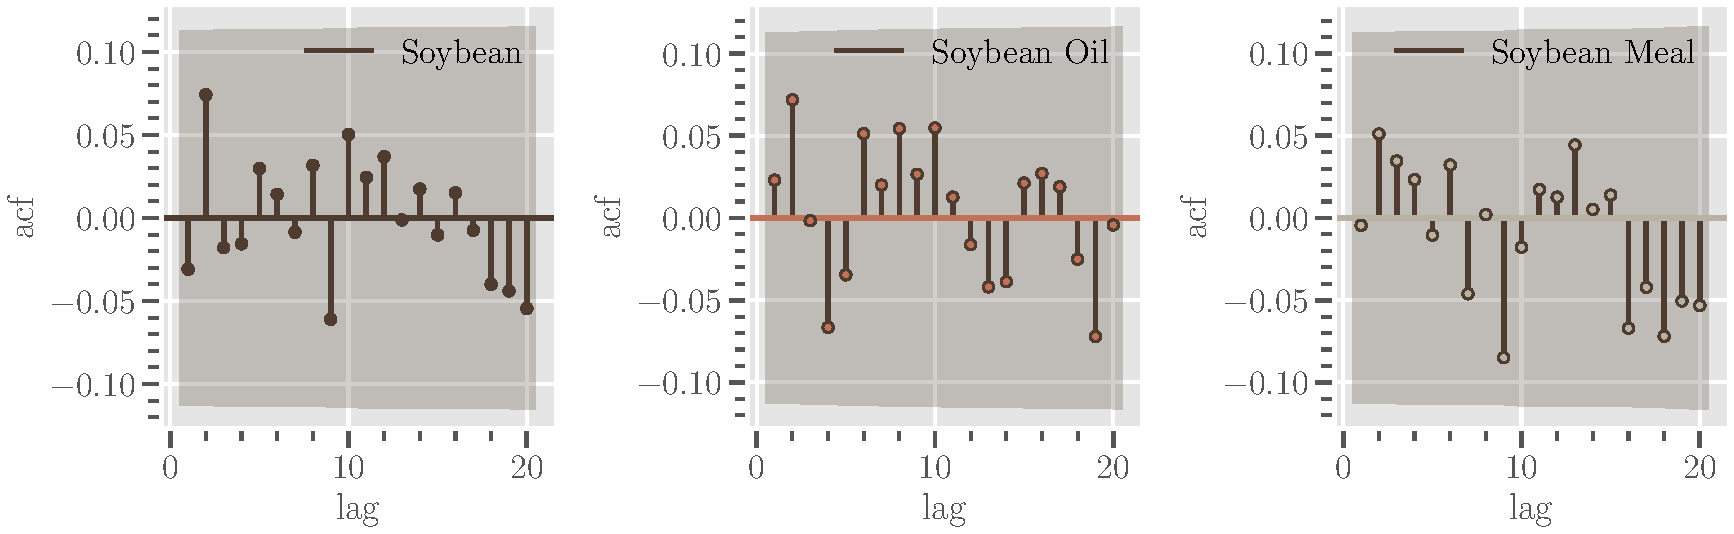
\includegraphics[width=\linewidth]{04_ACF}
	\caption{\textbf{Analiza szeregów czasowych (1/2).} Funkcje autokorelacji dla każdego aktywa. \label{fig:acf}}
\end{figure}

\begin{figure}[h]
	\centering
	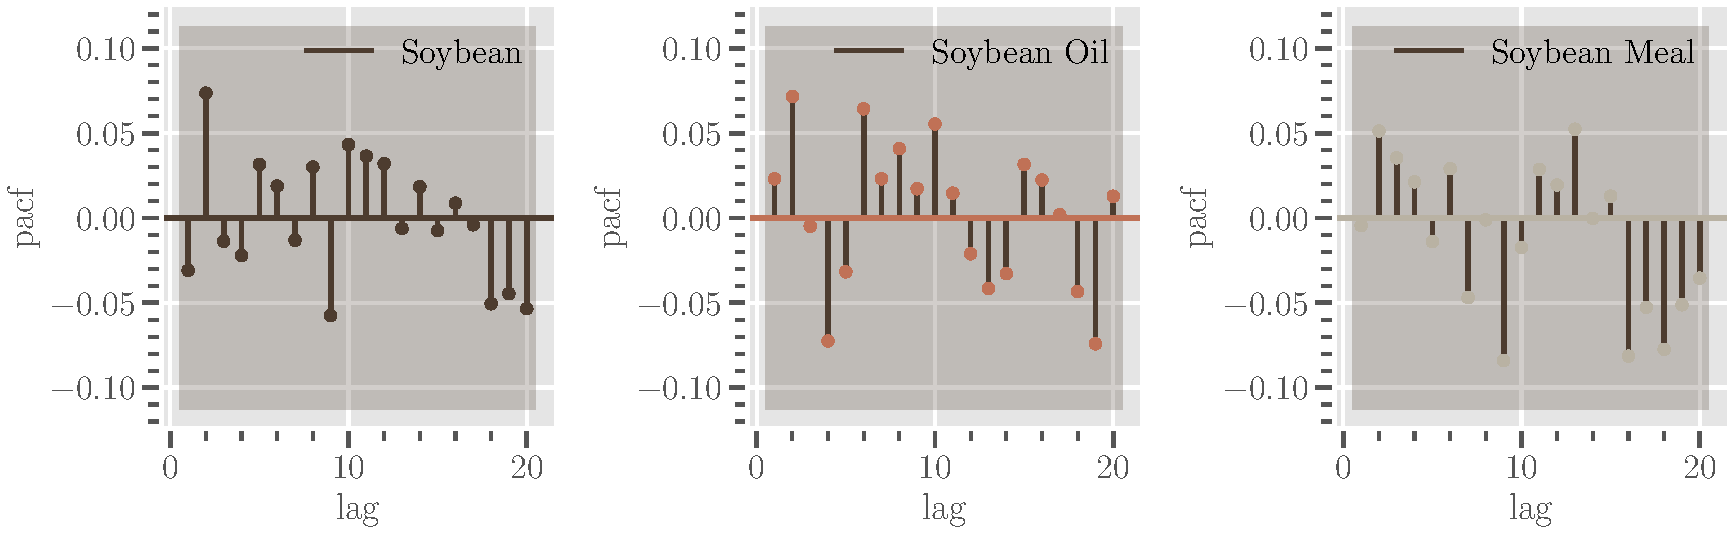
\includegraphics[width=\linewidth]{04_PACF}
	\caption{\textbf{Analiza szeregów czasowych (2/2).} Funkcje częściowej autokorelacji dla każdego aktywa. \label{fig:pacf}}
\end{figure}

\begin{table}
	\centering
	\csvreader[
	tabular=lcc,
	table head=\toprule \bfseries{Asset} & \bfseries{ADF~Test~Statistic} & \bfseries{p-value} \\\midrule,
	late after last line=\\\bottomrule % horizontal line at the end of the table
	]{
		Tables/Stationarity.csv
	}{}{\csvlinetotablerow}
	
	\caption{\textbf{Test stacjonarności szeregów czasowych.} Tabela przedstawia statystyki testowe i p-wartości testu \emph{Augmented Dickey-Fuller}. W każdym przypadku odrzucamy hipotezę zerową o niestacjonarności szeregów.
		\label{tab:adf_test}}
\end{table}

\FloatBarrier
\subsubsection{Część GARCH modelu}
W kolejnym kroku sprawdziliśmy homoskedastyczność szeregów czasowych. Dokonaliśmy wizualnej inspekcji wykresów odchylenia standardowego logzwrotów dla każdego aktywa przy pomocy ruchomego okna o długości $8$ tygodni. Rysunek \ref{fig:homoskedasticity} prezentuje przykład takiego wykresu dla cen soi. Widać na nim, że zmienność nie jest stała, lecz ma oscylujący okresowy charakter. Aby uchwycić tę informację użyliśmy modelu GARCH(m, n) opisanego równaniem \ref{eq:garch_part}. Modele były dopasowywane dla każdego aktywa osobno, za pomocą metody SLSQP (sequential least squares programming) wbudowanej w pakiet \emph{arch}, a następnie porównywane zostały pod względem kryterium informacyjnego AIC. Finalny model GARCH(2,3) został wybrany na podstawie najniższego średniego AIC ze względu na wszystkie aktywa. Wartości AIC, oraz wyniki kalibracji GARCH(2,3) zawarte są w tabelach odpowiednio: \ref{tab:garch_choice} oraz \ref{tab:garch_fit}.

\begin{figure}[h]
	\centering
	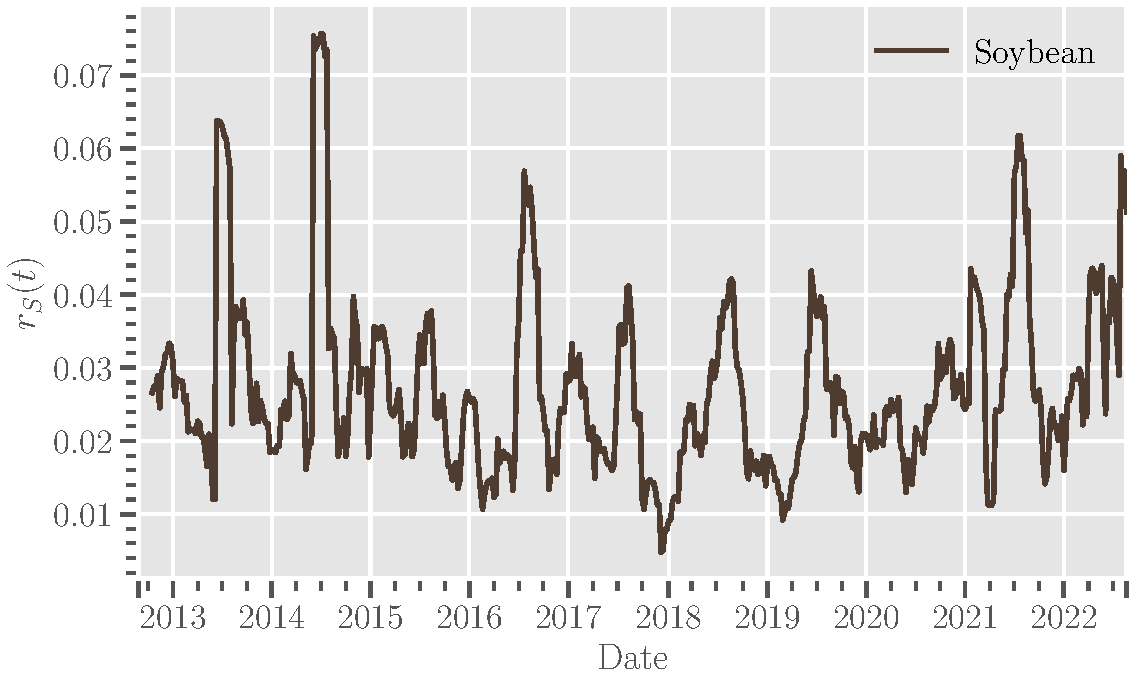
\includegraphics[width=0.7\linewidth]{04_Heteroskedasticity}
	\caption{\textbf{Analiza homoskedastyczności.} Wykres odchylenia standardowego logzwrotów cen spot soi na ruchomym oknie o długości 8 tygodni. \label{fig:homoskedasticity}}
\end{figure}

\begin{table}
	\centering
	\csvreader[
	tabular=cc|ccc|c,
	table head=\toprule \bfseries{m} & \bfseries{n} & \bfseries{Soybean} & \bfseries{Soybean Oil} & \bfseries{Soybean Meal} & \bfseries{Average} \\ \midrule,
	late after last line=\\ \bottomrule% horizontal line at the end of the table
	]{
		Tables/GARCH_choice.csv
	}{}{\csvlinetotablerow}
	
	\caption{\textbf{Wybór modelu GARCH(m,n).} Wartości kryterium AIC dla różnych wartości $m$ i $n$ dopasowywanych modeli GARCH, posortowane rosnąco wzgledem średniego AIC. \label{tab:garch_choice}}
\end{table}

\begin{table}
	\centering
	\csvreader[
	tabular=r|cccc,
	late after line=,
	table head=\toprule \bfseries{Asset} & \bfseries{Parameter} & \bfseries{Value} & \bfseries{Std. Error} & \bfseries{t-statistic},
	before line = \ifthenelse{\equal{\csvcolii}{$\mu$}}{\\ \midrule}{\\},
	table foot = \\ \bottomrule
	]{
		Tables/GARCH_fit.csv
	}{}{\csvlinetotablerow}
	
	\caption{\textbf{Parametry modeli GARCH(2,3).} Tabela przedstawia dopasowane wartości średniej logzwrotów $\mu$, oraz parametrów modelu GARCH(2,3) dla każdego aktywa. \label{tab:garch_fit}}
\end{table}

Finalnie, otrzymaliśmy szeregi czasowe reziduów $e_{i,t}$, które według czwartego równania założonego modelu \ref{eq:model_armagarch} powinny być niezależne od siebie, oraz scentrowane o jednostkowej wariancji. Przeprowadziliśmy więc testy: Ljunga-Boxa, t, oraz chi kwadrat aby sprawdzić hipotezy zerowe niezależności, średniej równej zero i wariancji równej jeden. Wyniki zaprezentowane w tabeli \ref{tab:iid_01_test} pokazują, że w przypadku żadnego aktywa nie udało się odrzucić powyższych hipotez.

\begin{table}
\begin{adjustbox}{width=\columnwidth, center}	
	\centering
	\csvreader[
	tabular=r|cccccc,
	table head=\toprule  & \multicolumn{2}{c}{\bfseries{Soybean}} & \multicolumn{2}{c}{\bfseries{Soybean Oil}}  & \multicolumn{2}{c}{\bfseries{Soybean Meal}}  \\ 
	\bfseries{Test} & \bfseries{Test statistic} & \bfseries{p-value} & \bfseries{Test statistic} & \bfseries{p-value} & \bfseries{Test statistic} & \bfseries{p-value}\\\midrule,
	late after last line=\\\bottomrule % horizontal line at the end of the table
	]{
		Tables/IID01Test.csv
	}{}{\csvlinetotablerow}
	
\end{adjustbox}
	\caption{\textbf{Testy IID(0,1) reziduów.} Tabela przedstawia statystyki testowe i p-wartości testów: \emph{Ljunga-Boxa} (na niezależność), \emph{t testu} (średnia próbki równa 0) oraz $\chi^2$ (wariancja próbki równa 1) dla reziduów modeli GARCH(2,3).  W przypadku testu Ljunga-Boxa podano wartości dla lagu o najmniejszej p-wartości.\label{tab:iid_01_test}}
\end{table}

\FloatBarrier
\subsubsection{Część Vine Copula modelu}

Mając szeregi czasowe reziduów będące $IID(0,1)$, możemy dopasować kopułę do struktury zależności między nimi. Rezidua najpierw zostały przetransformowane poprzez transformację PIT (\ref{def:PIT}) opartą o ich empiryczne dystrubuanty, co przedstawia rysunek \ref{fig:ecdf_pit}. Rysunek \ref{fig:pair_copulas} ukazuje natomiast zależności pomiędzy poszczególnymi ujednostajnionymi reziduami do której będziemy dopasowywać rozkład Vine Copula.

\begin{figure}[h]
	\centering
	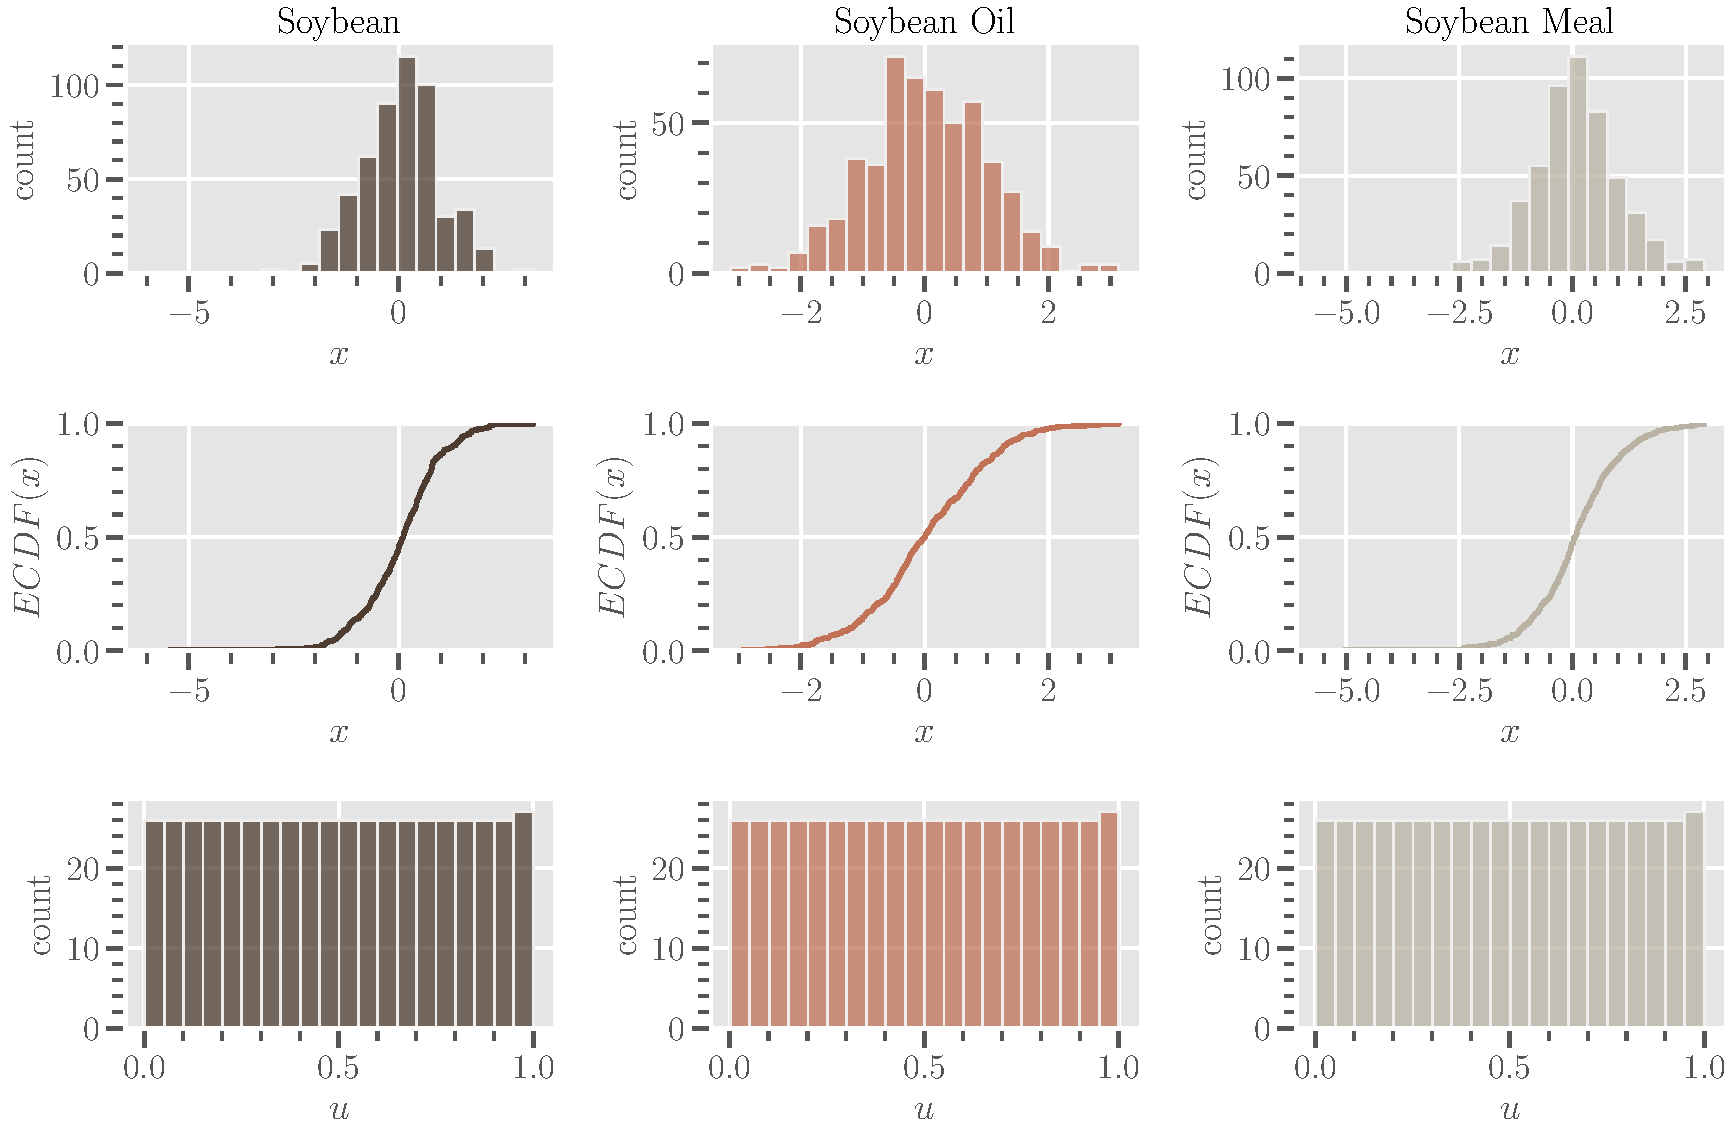
\includegraphics[width=\linewidth]{04_ECDFs}
	\caption{\textbf{Transformacja PIT.} Histogramy rezidów (górny panel), empiryczne dystrybuanty (środkowy panel) i rezidua przetransformowane poprzez PIT (dolny panel). \label{fig:ecdf_pit}}
\end{figure}

\begin{figure}[h]
	\centering
	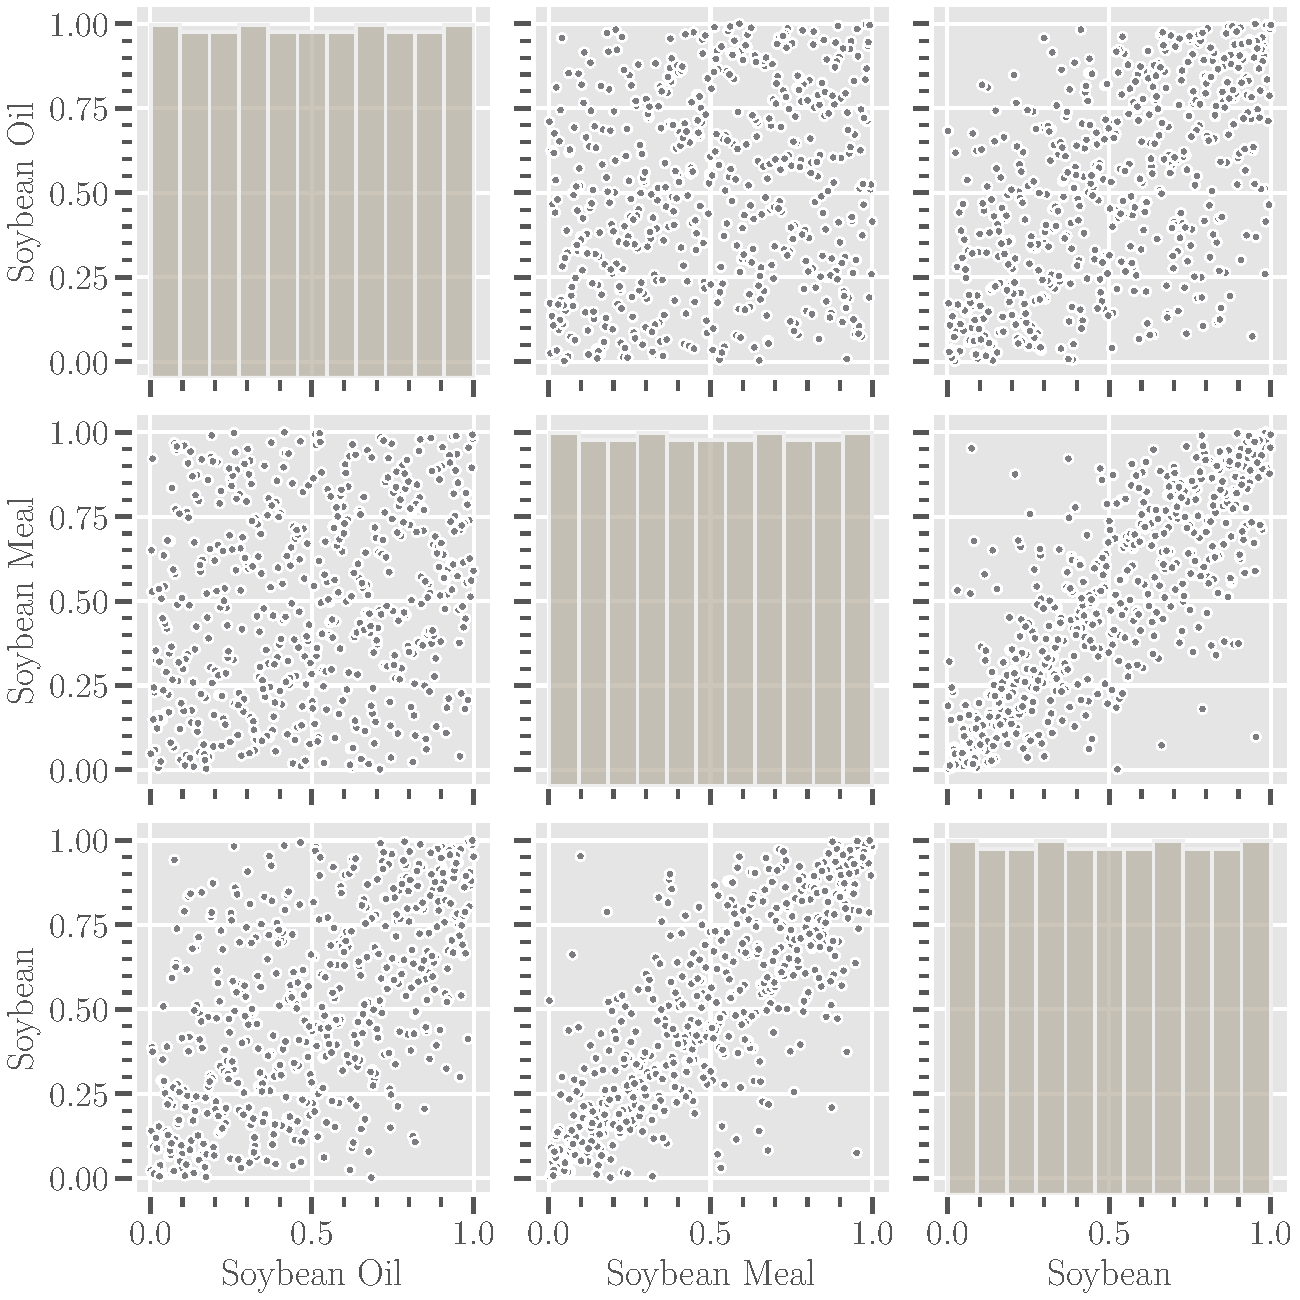
\includegraphics[width=0.9\linewidth]{04_PairPlotCopulaScale}
	\caption{\textbf{Struktura zależności reziduów.} Wykresy punktowe każdy-z-każdym, oraz histogramy reziduów. \label{fig:pair_copulas}}
\end{figure}

Wybór odpowiedniej Vine Copula oznacza wybór rodzaju struktury (R-vine, D-vine, C-vine, $\dots$), wybór dwuwymiarowych kopuł wewnątrz struktury, oraz estymację ich parametrów. Jak pokazaliśmy w przykładzie \ref{subsub:przyklad_3_wymiary}, w przypadku $3$-wymiarowych danych R-vine jest w stanie przyjąć jedynie jednen rodzaj struktury, który jednocześnie spełnia warunki na C-vine oraz D-vine. Dodatkowo widzieliśmy, że cała struktura zależy jedynie od kolejności zmiennych w pierwszym drzewie $T_1$.  Problem redukuje się tu więc do wyboru odpowiedniej kolejności, oraz estymacji dwuwymiarowych kopuł w takiej strukturze.\\
Używamy tu algorytmu podanego w \cite{Dissmann_Vines}, który dobiera strukturę w sposób krokowy: zaczyna od pary najsilniej związanych ze sobą zmiennych i rozszerza strukturę w każdym kroku, wykorzystując $\tau$ Kendalla w celu dokonywania lokalnie optymalnych decyzji. Tabela \ref{tab:vine_selection} prezentuje wyniki tej estymacji dla różnych kolejności drzewa $T_1$ - algorytm Dissmanna wskazuje na wybór struktury o kolejności zmiennych $132$. Zwracamy uwagę na obserwację, że struktury o odwrotnych kolejnościach (jak $132$ i $231$) mają tę samą wartość AIC oraz log-likelihood. Wynika to z faktu, że gdy algorytm Dissmanna poszukuje optymalnej decyzji w danym kroku (czyli poszukuje odpowiednich dwuwymiarowych kopuł), pozwalamy mu na poruszanie się w dziedzinie kopuł przedstawionych w rozdziale \ref{subsec:dwuwymiarowe_kopuly_przyklady} które są (radialnie) symetryczne. Z tego powodu grafy struktury D-vine nie są grafami skierowanymi i kolejność w drzewach można bez konsekwencji odwracać. Skupienie na kopułach radialnie symetrycznych jest popularnym podejściem w praktyce (\cite{Cherubini_Copula_Methods_in_Finance}, \cite{Czado_Vine_Copulas}), a rysunek \ref{fig:pair_copulas} pokazuje że w przypadku naszych danych nie ma przesłanek do podejrzewania asymetrycznych zależności (obrót wykresów punktowych względem osi $x=y$ nie powoduje zmiany charakteru zależności - są one radialnie symetryczne). O asymetrycznych kopułach przeczytać można więcej w \cite{BedfordCooke2002}.\\
Dodatkowo ponieważ poruszamy się w dziedzinie kopuł \emph{parametrycznych}, możemy przyspieszyć algorytm Dissmanna wykorzystując $\tau$ Kendalla do dopasowania dwuwymiarowych kopuł. Ta statystyka i tak jest obliczana w każdym kroku dla każdej pary zmiennych w celu wybrania najsilniej związanych zmiennych, więc algorytm może o razu użyć zależności wymienionych w \ref{subsec:dwuwymiarowe_kopuly_przyklady} do przełożenia $\hat{\tau}$ na $\hat{\Theta}$, czyli parametry konkretnej rodziny kopuł. Klasyczną alternatywą do estymacji parametrów byłaby metoda największej wiarogodności (\cite{BedfordCooke2002}, \cite{Czado_Vine_Copulas}).\\

\begin{table}
	\centering
	\csvreader[
	tabular=r|cc,
	table head=\toprule \bfseries{$T_1$ order} & \bfseries{AIC} & \bfseries{Log-likelihood} \\ \midrule,
	table foot = \bottomrule
	]{
		Tables/VineAICs.csv
	}{}{\csvlinetotablerow}
	
	\caption{\textbf{Wybór struktury Vine Copula.} Wartości kryterium AIC oraz log-likelihood dla finalnego modelu, w zależności od kolejności pierwszego drzewa. \label{tab:vine_selection}}
\end{table}

Dopasowana w ten sposób struktura zaprezentowana jest na rysunku \ref{fig:vine_fit}. Widzimy w niej użycie kopuł: Gaussowskiej i Franka to modelowania zależności między reziduami. Obie te kopuły modelują zależności symetryczne i nie posiadają współczynnika zależności ogonów. Co ciekawe, rezidua soi zostały wskazane na środkowym miejscu $T_1$. Jako że tę strukturę można traktować z perspektywy C-vine, to jej \emph{root node} (tutaj: soję) interpretować można jako najsilniejszy/najbardziej wpływowy wymiar (\cite{Czado_Vine_Copulas}), co zgadza się z intuicją.\\

\begin{figure}[h]
	\centering
	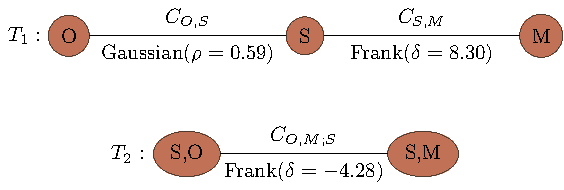
\includegraphics[width=0.8\linewidth]{04_FittedStructure}
	\medskip
	\begin{minipage}{\linewidth}
		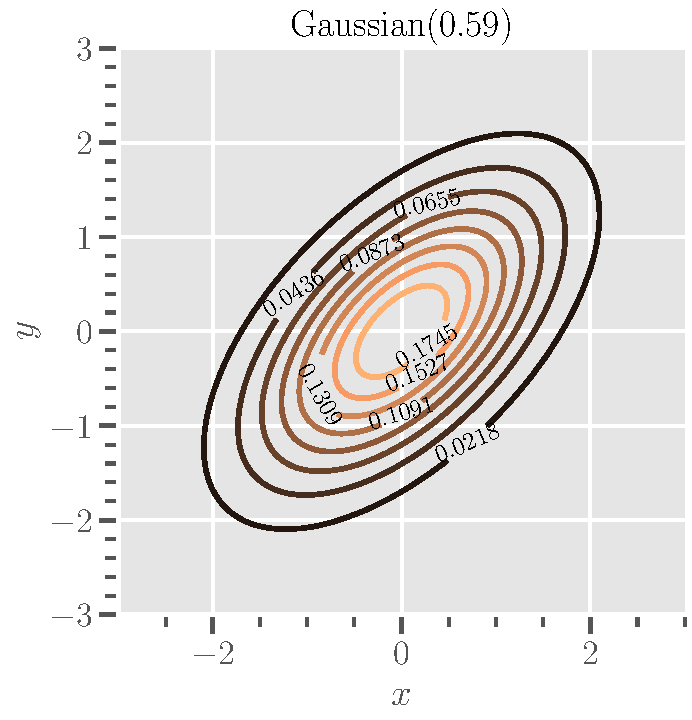
\includegraphics[width=0.45\linewidth]{04_Fitted_Soybean Oil_Soybean_contour_norm}
		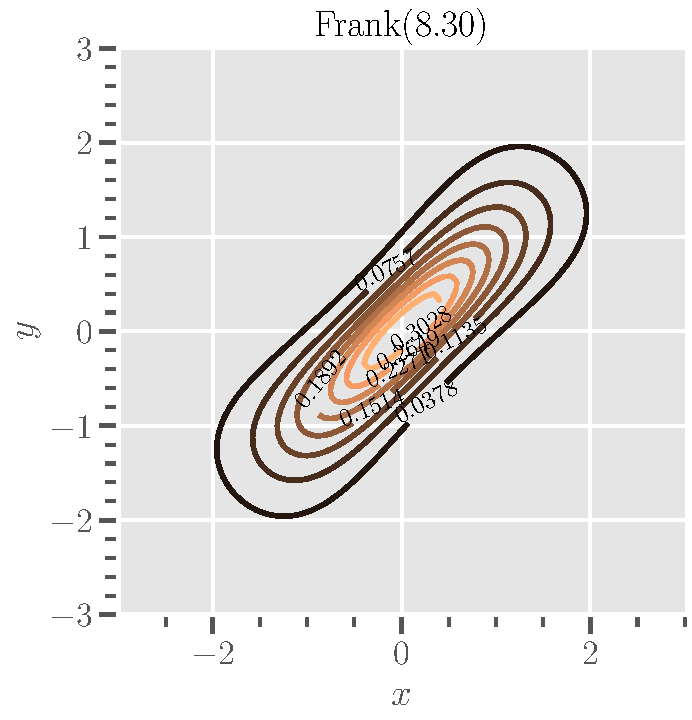
\includegraphics[width=0.45\linewidth]{04_Fitted_Soybean_Soybean Meal_contour_norm}
	\end{minipage}
	\begin{minipage}{\linewidth}
		\centering
		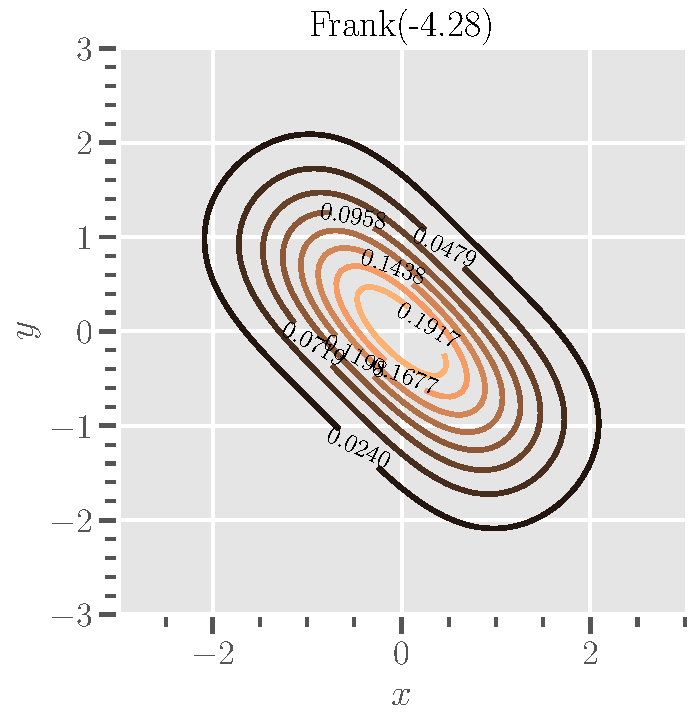
\includegraphics[width=0.45\linewidth]{04_Fitted_conditional_contour_norm}
	\end{minipage}
	\caption{\textbf{Model struktury zależności.} R-vine dopasowana do danych przy pomocy algorytmu Dissmanna. Graf struktury (górny panel) i kontury kopuł w skali brzegowo-znormalizowanej (dolny panel). \label{fig:vine_fit}}
\end{figure}
\FloatBarrier